\title{Singularity Software}
\date{\today}

\documentclass[12pt]{article}
\usepackage[a4paper]{geometry}
\usepackage{makeidx}
\usepackage[acronym]{glossaries}
\usepackage{lscape}
\usepackage{amsmath}
\usepackage{graphicx}
\usepackage[final]{pdfpages}
% \usepackage{hyperref} % Makes links from ToC

\geometry{top=1.0in, bottom=1.0in, left=1.0in, right=1.0in} % Sets the margins

\setlength{\parindent}{0pt} % Fixes the paragraph spacing problem

% This is all for formatting and making the Table of Contents according to 
% spec. Don't play with it.
\makeatletter
\renewcommand\l@section[2]{%
  \ifnum \c@tocdepth >\z@
    \addpenalty\@secpenalty
    \addvspace{1.0em \@plus\p@}%
    \setlength\@tempdima{1.5em}%
    \begingroup
      \parindent \z@ \rightskip \@pnumwidth
      \parfillskip -\@pnumwidth
      \leavevmode \bfseries
      \advance\leftskip\@tempdima
      \hskip -\leftskip
      #1\nobreak\ 
      \leaders\hbox{$\m@th\mkern \@dotsep mu\hbox{.}\mkern \@dotsep mu$}
     \hfil \nobreak\hb@xt@\@pnumwidth{\hss #2}\par
    \endgroup
  \fi}
\makeatother

\makeindex

% Construct the glossary here
% Use the template below, then where the word appears (in the case below, computer), replace computer with \gls{computer}
\makeglossaries

\newglossaryentry{Sifteo Cubes}
{
  name={Sifteo Cubes},
  description={are small machines capable of loading programs and interacting with one another as well as responding to predefined movements}
}

\newglossaryentry{Object-Oriented Programming}
{
  name={Object-Oriented Programming},
  description={is a programming paradigm using objects to design applications}
}

\newglossaryentry{Windows}
{
  name={Windows},
  description={is a series of operating systems developed by Microsoft}
}

\newglossaryentry{Mac}
{
  name={Mac},
  description={is a series of lines of personal computers developed by Apple}
}

\newglossaryentry{Linux}
{
  name={Linux},
  description={is a Unix-based operating system based on free and open source software}
}

\newglossaryentry{cross-platform support}
{
  name={cross-platform support},
  description={is an attribute given to software implemented and operable on multiple computer platforms}
}

\newacronym{API}{API}{\glsadd{API}{Application Programming Interface}}

\newglossaryentry{APIg}
{
  name={Application Programming Interface},
  description={is an interface implemented by a software program that enables it to interact with other software}
}


\newglossaryentry{open source}
{
  name={open source},
  description={is an attribute given to software for which the source code is freely available}
}

\newacronym{IDE}{IDE}{\glsadd{IDE}{Integrated Development Environment}}

\newacronym{SDK}{SDK}{\glsadd{SDK}{Software Development Kit}}

\newglossaryentry{SDKa}
{
  name={Software Development Kit},
  description={is a collection of tools designed to help build software for a particular platform. It may include an \index{API} and an emulator of the target platform among other things.}
}

\newglossaryentry{IDEa}
{
  name={Integrated Development Environment},
  description={is software that provides a comprehensive work environment for computer programmers and software developers}
}


\newacronym{GUI}{GUI}{\glsadd{GUI}{Graphical User Interface}}

\newglossaryentry{GUIa}
{
  name={Graphical User Interface},
  description={is a visual way of allowing the user to interace with a computer program}
}

\newglossaryentry{version control}
{
  name={version control},
  description={is the management of documents and programs for a project over many versions in a well-organized manner}
}

\newglossaryentry{issue tracking system}
{
  name={issue tracking system},
  description={is a piece of software used to maintain a list of issues as generated during a project}
}

\newglossaryentry{usability study}
{
  name={usability study},
  description={is a manner of evaluating the design and user experience of a product by testing it on users}
}

\renewcommand*\arraystretch{1.5}

\begin{document}
\vspace*{\fill}
        \begin{center}
                \LARGE{Siftables Emulator} \\
                \LARGE{\textit{Singularity Software}} \\
                \vspace{.15in}
                \large{\today} \\
                \vspace{4in}
                        Alex Mullans \\
                        Ethan Veatch \\
                        Eric Vernon \\
                        Kurtis Zimmerman
        \end{center}
\vspace*{\fill}
\thispagestyle{empty}

\clearpage

\tableofcontents

\clearpage

\section{Introduction}
Developers of applications for the \gls{Sifteo Cubes}\index{Sifteo} currently must test programs they create for the platform on the Cubes themselves.  With a full release of the Cubes and corresponding \gls{API}\index{API}\glsadd{APIg} still pending, developers unable to join the Sifteo Early Access program are left without a software-based interface within which to productively develop Sifteo programs. As such, Singularity Software will provide, in the form of the Siftables Emulator, a software-based emulator\index{emulator} for the Sifteo Cubes that will allow any developer to try programming in the unqiue environment provided by the Cubes.\\\\
This document summarizes a series of milestone documents that accompany the planning of the Siftables\index{Siftables} Emulator\index{emulator}.

\section{Client Background}
Clients Tim Ekl and Eric Stokes are alumni of Rose-Hulman. Mr. Ekl is currently working on a M.S. degree in Engineering Management; Mr. Stokes is currently working for n{\raise.17ex\hbox{$\scriptstyle\sim$}}ask Signal Processing Systems in Denver, Colorado. As former Rose-Hulman students, the clients are avid users of technology who follow new trends in the industry. As a result of this interest in new technology, both Mr. Stokes and Mr. Ekl discovered and purchased Sifteo Cubes\index{Sifteo Cubes}, a revolutionary product that consists of a set of (anywhere from 1 to 6) mini computers. While both clients have a set of 3 Sifteo Cubes, they realized that not everyone interested in the project could have the luxury of physical hardware to work with. As such, they asked Singularity Software---via the Junior Project proposal process at Rose-Hulman---to construct a software emulator\index{emulator} for the Cubes that would make the development of Sifteo\index{Sifteo} applications easier, especially in the testing phase.

\clearpage

\section{Current System}
Currently the only system available to developers is the Siftulator, the emulator released in Sifteo's SDK.  It allows for emulation of all Cube manipulations, and the numebr of Cubes can be increased or reduced through the interface.  An API is available through the Sifteo website, and several example games have been written for use in the emulator workspace.  The Siftulator only runs on Windows machines, leaving it inaccessible to some users.  A screenshot, taken from Sifteo's developer website, is shown below.
\begin{center}
        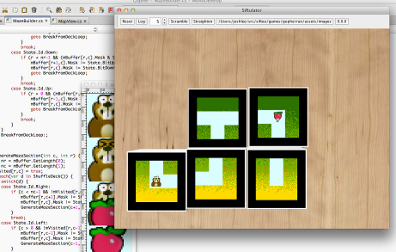
\includegraphics{siftulator.png}
\end{center}

\section{User/Stakeholder Description}

               \subsection{User/Stakeholder Profiles}

                          \subsubsection{Sifteo application developers}
                          As the primary target audience of the system, developers targeting the Sifteo\index{Sifteo} platform are assumed to have a reasonable amount of technical background; they are not novice computer users and are familiar with programming concepts like \gls{Object-Oriented Programming}\index{Object-Oriented Programming} and \gls{API}\index{API}s. As developers may hail from platforms ranging from \gls{Windows} to \gls{Mac} to \gls{Linux}, \gls{cross-platform support} is an important consideration.\\\\
                          Possible problems for this user type include an unstable or crash-prone system: as developers are writing and testing their own code, it is essential that the emulator\index{emulator} does not contribute to the failures that the user must debug. Developers will deem the emulator\index{emulator} project a success when they can successfully program and test software that uses any or all of the features of the Sifteo\index{Sifteo} cubes on their development platform.

                          \subsubsection{Clients}
                          The clients (Tim Ekl and Eric Stokes) are assumed to be a subset of the Sifteo\index{Sifteo} application developers user class. However, their programming knowledge and knowledge of the Sifteo\index{Sifteo} Cubes\index{Sifteo Cubes} is known to be more advanced than that of the average application developer. As such, their needs require that the emulator\index{emulator} is capable of being pushed to the same limits as the actual platform.

                          \subsubsection{Singularity Software}
                          Singularity Software, as the team behind Siftables\index{Siftables} Emulator\index{emulator}, is primarily interested in the creation of a finished product that can be delivered to the clients at the conclusion of the Rose-Hulman junior project cycle. As a team, we are less familiar with the Sifteo platform and are also relatively inexperienced with the scale of project the emulator\index{emulator} entails.

                          \subsubsection{Sriram Mohan (CSSE Department)}
                          As the advisor of the Junior Project, Dr. Mohan has a vested interest in the creation of a finished, deliverable product. His key responsibility is to review documents created within the scope of the Junior Project series of courses.

               \subsection{User Environments}

                          \subsubsection{Sifteo application developers}
                          The typical Sifteo application developer may be working on his own, or he may be working with a team of developers; he or they will be working on workstations or powerful development laptops that have a significant amount of graphics horsepower. They may or may not be connected to the Internet during development, depending on the location in which they are developing. Additionally, they may be \gls{Windows}, \gls{Mac}, or \gls{Linux} users and will be using various \glspl{IDE}\glsadd{IDEa} specific to their platform; integration between such \glspl{IDE} and the Siftables\index{Siftables} Emulator\index{emulator}, while possibly desirable, is not a requirement.

                          \subsubsection{Clients}
			  Mr. Stokes and Mr. Ekl are both primarily \gls{Mac} users, although both clients also own and occasionally use \gls{Windows} machines as well. Their environment is essentially the same as that of the typical Sifteo\index{Sifteo} application developer.

               \subsection{Key Needs}

                          \subsubsection{Emulate Sifteo Cubes in a desktop GUI application}
                          No emulator currently exists for the Sifteo\index{Sifteo} platform; the need is currently either filled by homebrew efforts like Mr. Ekl's Java-based emulator\index{emulator}, or circumvented by using the Cubes themselves as a testing platform. The clients envision a solution where all of the interactions possible with a set of Early Access Sifteo Cubes can be replicated in a software emulator\index{emulator}.

                          \subsubsection{Develop an API for creating applications in the emulator’s Cubes}
                          An \gls{API}\index{API} is necessary to facilitate interaction with the virtual Sifteo Cubes. Currently, no \gls{API} has been made available by Sifteo for the physical cubes, and no emulator\index{emulator} \gls{API}\index{API} exists because no emulator\index{emulator} exists. The clients would like an \gls{API}\index{API} with which the virtual Cubes can be programmed. Mr. Ekl stipulated that shadowing the official Sifteo \gls{API}\index{API}, while potentially beneficial for long-term development, is not a requirement.

                          \subsubsection{Showcase Cube/emulator functionalities with samples}
                          Sifteo currently provides example games that run on the Cubes as a showcase of what the platform can achieve and what unique features it can offer to the user. The clients would like to have a similar showcase available for the emulator as an aid in understanding both the emulator platform and the larger Sifteo Cubes\index{Sifteo Cubes} programming platform.

              \subsection{Alternatives \& Competition}
              Singularity Software's Siftables Emulator\index{emulator} will be the first software of its kind for the Cubes. The only true competition is the Sifteo Cubes themselves. The Cubes have the advantage of physicality---as tactile objects, they will always be superior in terms of user experience when compared to an emulator. However, they are expensive and only manufactured in limited quantities at the moment; the Siftables Emulator\index{emulator} is, by contrast, infinitely available as an \gls{open source}\index{open source} piece of software.

\section{Product Overview}

              \subsection{Product Perspective}
              Siftables Emulator\index{emulator} is a free independent system used to emulate the way Sifteo Cubes handle motions and interactions.

              \subsection{Elevator Statement}
              Due to the limited availability of Sifteo Cubes, developers unable to obtain a set of Cubes have no good way to test the programs they create for the platform. At Singularity Software, our goal is to develop an emulator\index{emulator} for the Cubes that will be able to emulate an arbitrary number of Sifteo Cubes\index{Sifteo Cubes} and the way they handle physical motions and interactions. Along with the emulator itself, Singularity will develop an \gls{API}\index{API} and example games and programs.
\clearpage
              \subsection{Summary of Capabilities}
              The main features of our emulator\index{emulator} work together to allow developers to quickly start Sifteo application development by making a virtual edition of the Cubes available for emulation and testing.
              \begin{table}[h]
                \begin{tabular}{p{3in} | p{3in}}
                  \textbf{Feature} & \textbf{Benefit} \\ \hline
                  Workspace where multiple cubes can be emulated
                            & A user-friendly way to develop for multiple cubes \\ \hline
                  Buttons and gestures to control the cubes
                            & An easier way to control the basic movements of the cubes in place of physical manipulations \\ \hline
                  Ability to load programs into the cubes
                            & Allows the user to test his own programs and example programs in the emulator \\ \hline
                  Example games (requirement)
                            & Gets new emulator\index{emulator} users started with the platform \\ \hline
                  \Gls{open source}\index{open source}  (requirement)
                            & Allows the community to contribute improvements to the emulator\index{emulator} \\ \hline
                  \gls{API}\index{API} (requirement)
                            & A standard way of interacting with the virtual Cubes
                \end{tabular}
              \end{table}

              \subsection{Assumptions and Dependencies}
              Sifteo\index{Sifteo} has plans to release an \gls{API}\index{API} of their own for the Cubes; Singularity will attempt to make our \gls{API}\index{API} shadow much of the language and functionality of the official Sifteo \gls{API}\index{API}. 

              \subsection{Estimate of Cost}
			  Because it is an \gls{open source} piece of software, Singularity Software does not believe that the Siftables Emulator\index{emulator} will incur any monetary costs throughout the project.
\clearpage

\section{Features}
Six attributes accompany each feature described below: 
    \begin{description}
        \item[Status:] a  measure of the feature's progress duing the project definition period, either \textit{Proposed} or \textit{Approved}
        \item[Priority:] the relative importance of each feature, either \textit{Useful}, \textit{Important}, or \textit{Critical}
        \item[Risk:] the probability that the feature will bring about undesirable events, either \textit{Low}, \textit{Medium}, or \textit{High}
        \item[Stability:] the probability that the feature will change, either \textit{Low}, \textit{Medium}, or \textit{High}
        \item[Reason:] the source of the required feature
        \item[Effort:] an estimate of the relative amount of work required to complete the feature, either \textit{Low}, \textit{Medium}, or \textit{High}
    \end{description}
    The features are outlined in the table on the following page.
    \begin{landscape}
    \begin{table}[h]
      \begin{tabular}{p{1.5in} | p{1.75in} | p{.75in} | p{.75in} | p{.75in} | p{.75in} | p{1.75in} | p{.6in}}
        \textbf{Feature} &
        \textbf{Description} &
        \textbf{Status} &
        \textbf{Priority} &
        \textbf{Risk} &
        \textbf{Stability} &
        \textbf{Reason} &
        \textbf{Effort} \\ \hline

        Individual, virtual Sifteo Cube &
        A virtual representation of a single Sifteo cube &
        Approved &
        Critical &
        Low &
        High &
        Replicates physical Sifteo Cube &
        Medium \\ \hline

        Buttons to manipulate each virtual Cube &
        Buttons on the virtual Cube will allow the user to flip and tilt it &
        Approved &
        Critical &
        Medium &
        High &
        Replaces physical actions where said actions would be impractical with a mouse &
        Medium \\ \hline

        Workspace where multiple cubes can be emulated &
        Multiple cubes will be displayed on a workspace that replicates the free-form nature of physical Sifteo Cubes\index{Sifteo Cubes} &
        Approved &
        Critical &
        Low &
        High &
        Replicates multiple Sifteo Cubes\index{Sifteo Cubes} in a natural, free-form environment &
        High \\ \hline

        Interactions between Cubes &
        The Cubes present on the workspace will communicate when they are neighbored &
        Approved &
        Critical &
        Low &
        High &
        Cubes can simulate the interactions possible with physical Cubes &
        High \\ \hline

        Load programs into the Cubes &
        The user will load his own and example programs into the emulator’s\index{emulator} Cubes &
        Approved &
        Critical &
        Medium &
        High &
        The ability to program programs for the emulator\index{emulator} is dependent on a common interface &
        High \\ \hline

        Snap Cubes to invisible grid &
        The Cubes will snap into an invisible grid when a button is clicked &
        Proposed &
        Useful &
        Medium &
        High &
        Increases productivity by allowing a quick reset if the Cubes are in disarray &
        Low \\ \hline

        Zoom Workspace &
        The Workspace will zoom to the level of an individual Cube or the whole space &
        Proposed &
        Useful &
        Low &
        High &
        Inspecting individual Cubes allows for precise checks of program \glspl{GUI}\index{GUI}\glsadd{GUIa} &
        Low \\ \hline

      \end{tabular}
    \end{table}
    \end{landscape}

\section{Constraints}
        While much of this project is open-ended, there are a few basic constraints. At the direction of the clients, all code should be \gls{open source}\index{open source} and version-controlled\glsadd{version control}. Mr. Ekl requested that the emulator run easily on \gls{Mac} as well as \gls{Windows}, with the stipulation that \gls{Linux} compatibility would satisfy the \gls{Mac} requirement for Singularity's testing purposes. In addition, the clients requested that an \gls{issue tracking system} be put in place and used throughout the development process. Finally, the emulator\index{emulator} must be completed by May 18th---the end of Spring Quarter 10th week---to satisfy the requirements of the clients and of Dr. Mohan.

\section{Use Cases}

  \subsection{Load program}

    \begin{description}
      \item[Name:] Load program
      \item[Description:] The User selects the program file to be loaded and run by the emulator\index{emulator}.
      \item[Actors:] User
      \item[Basic flow:] \hfill 
        \begin{enumerate}
	  \item{The User presses the ``Load a program" button.}
	  \item{The User selects a *.siftem file in the file dialog.}
	  \item{The User presses ``Open" button.}
	  \item{The emulator loads the selected program on the Cubes in the emulator.}
        \end{enumerate}
      \item[Alternate flows:] \hfill \\
	When the User opens an incompatible file (i.e. any file without the .siftem extension),
        \begin{enumerate}
			\item{An error dialog is presented to the User with the message: "The selected file is not a .siftem emulator file and cannot be loaded."}
			\item{The use case terminates and no program is loaded.}
        \end{enumerate}
	When the User opens a corrupt or otherwise unloadable file,
        \begin{enumerate}
			\item{An error dialog is presented to the User with the message: "The selected file is corrupt and cannot be loaded."}
			\item{The use case terminates and no program is loaded.}
        \end{enumerate}
	When the User presses the ``Cancel" button:
        \begin{enumerate}
			\item{The use case terminates and no program is loaded.}
        \end{enumerate}
	When the User is already running a program,
		\begin{enumerate}
			\item{A warning dialog is presented to the User with the message: "Loading this program will clear all data from the previous program run. Proceed?"}
			\item{If the User presses ``Yes" on the warning dialog, flow returns to Step 2 of the basic flow.}
		\end{enumerate}
	When the User presses ``No" on the warning dialog:
        \begin{enumerate}
          \item{The use case terminates and the program is not reloaded.}
        \end{enumerate}
      \item[Pre-conditions:] \hfill
        \begin{enumerate}
          \item{The emulator is running.}
        \end{enumerate}
      \item[Post-conditions:] \hfill
        \begin{enumerate}
	  \item{The program is loaded or the User cancelled loading.}
        \end{enumerate}
      \item[Special requirements] \hfill
        \begin{enumerate}
          \item{The emulator should indicate that loading the program is in progress.}
          \item{The emulator should indicate when the program is finished loading.}
        \end{enumerate}
    \end{description}
%\newpage
  \subsection{Reload program}

    \begin{description}
      \item[Name:] Reload program
      \item[Description:] The User reloads the program currently running in the emulator.
      \item[Actors:] User
      \item[Basic flow:] \hfill
        \begin{enumerate}
			\item{A warning dialog is presented to the User with the message: "Reloading this program will clear all data from the previous program run. Proceed?"}
			\item{If the User presses ``Yes" on the warning dialog, the Emulator loads the program onto the Cubes in the emulator.}
        \end{enumerate}
      \item[Alternate flows:] \hfill \\
	When the User presses ``No" on warning dialog:
        \begin{enumerate}
          \item{The use case terminates and the program is not reloaded.}
        \end{enumerate}
      \item[Pre-conditions:] \hfill
        \begin{enumerate}
	  \item{A program is loaded in the emulator.}
        \end{enumerate}
      \item[Post-conditions:] \hfill
        \begin{enumerate}
	  \item{The program is reloaded or the current program state remains on the Cubes.}
        \end{enumerate}
      \item[Special requirements:] \hfill
        \begin{enumerate}
          \item{The emulator should indicate that loading the program is in progress.}
	  \item{The emulator should indicate when the program is finished loading.}
        \end{enumerate}
    \end{description}

  \subsection{Zoom screen}

    \begin{description}
      \item[Name:] Zoom screen
      \item[Description:] The User zooms the Workspace to the desired level.
      \item[Actors:] User
      \item[Basic flow:] \hfill
        \begin{enumerate}
	  \item{The User adjusts the zoom slider.}
	  \item{The Emulator magnifies the Cubes in the emulator according to the zoom level.}
        \end{enumerate}
      \item[Alternate flows:] \hfill \\
	None
      \item[Pre-conditions:] \hfill
        \begin{enumerate}
          \item{The emulator is running.}
        \end{enumerate}
      \item[Post-conditions:] \hfill
        \begin{enumerate}
	  \item{The program running at the beginning of this use case, if any, is still running.}
        \end{enumerate}
	  \item[Special requirements:] \hfill
        \begin{enumerate}
		\item{The zoom slider moves in discrete increments. The lowest (and default) level shows the whole workspace and the highest level shows one Cube with the edges of the surrounding Cubes visible for context.}
		\end{enumerate}
    \end{description}	

  \subsection{Add/remove Cubes}

    \begin{description}
      \item[Name:] Add/remove Cubes
      \item[Description:] The User adjusts the number of Cubes present in the emulator.
      \item[Actors:] User
      \item[Basic flow:] \hfill
        \begin{enumerate}
	  \item{The User drags the ``Number of Cubes" slider or uses the up/down arrows on the spinbox to increment or decrement the number of available Cubes by one.}
	  \item{The emulator adds/removes Cubes in emulator and resets its Workspace.}
	  \item{If Cubes are to be removed, the emulator starts with the bottom right-most of the Cubes (at their current positions) and works left. If more Cubes are to be removed after the second row is depleted, the emulator again starts at the bottom right-most of the remaining Cubes.}
        \end{enumerate}
      \item[Alternate flows:] \hfill \\
	None
      \item[Pre-conditions:] \hfill
        \begin{enumerate}
	  \item{The emulator is running.}
        \end{enumerate}
      \item[Post-conditions:] \hfill
        \begin{enumerate}
	  \item{The number of Cubes has been adjusted to the number specified.}
	  \item{The running program, if any, is terminated.}
        \end{enumerate}
	  \item[Special requirements:] \hfill
        \begin{enumerate}
		\item{The ``Number of Cubes" slider moves in discrete increments. The leftmost level shows one Cube and the rightmost level shows six Cubes.}
		\end{enumerate}
    \end{description}

  \subsection{Snap Cubes to grid}

    \begin{description}
      \item[Name:] Snap to grid
      \item[Description:] The Users pulls the Cubes into a grid orientation.
      \item[Actors:] User
      \item[Basic flow:] \hfill
        \begin{enumerate}
	  \item{The User presses the ``Snap to Grid" button.}
	  \item{The Emulator moves the Cubes to a grid orientation based on their current positions. It will maintain the Cubes' positions relative to other Cubes while doing so.}
        \end{enumerate}
      \item[Alternate flows:] \hfill \\
	None	
      \item[Pre-conditions:] \hfill
        \begin{enumerate}
	  \item{The emulator is running.}
        \end{enumerate}
      \item[Post-conditions:] \hfill
        \begin{enumerate}
	  \item{The Cubes are arranged in a grid.}
        \end{enumerate}
    \end{description}

  \subsection{Manipulate Cube}

    \begin{description}
      \item[Name:] Manipulate Cube
      \item[Description:] The User manipulates a Cube by clicking the buttons or the Cube itself.
      \item[Actors:] User
      \item[Basic flow:] \hfill
        \begin{enumerate}
	  \item{The User double clicks on a Cube.}
	  \item{The Cube responds as if a screen click occured.}
        \end{enumerate}
      \item[Alternate flows:] \hfill
        \begin{enumerate}
	  \item{The User clicks on one of the buttons superimposed on the Cubes' edges.}
	  \item{The Cube executes the appropriate action (i.e. flips, rotates, or tilts).}
        \end{enumerate}
        \begin{enumerate}
          \item{The User drags a Cube next to another Cube.}
	  \item{Cube communicates (``neighbors") with the Cube(s) it is adjacent to.}
        \end{enumerate}
	  \item{The User ``shakes" a Cube back and forth with the mouse (i.e. he laterally moves the Cube back and forth several times).}
	  \item{The Cube responds as if shaken.}
      \item[Pre-conditions:] \hfill
        \begin{enumerate}
          \item{The emulator is running.}
        \end{enumerate}
      \item[Post-conditions:] \hfill
        \begin{enumerate}
	  \item{If a program is running, the emulator has updated its state based on the Cube's change.}
        \end{enumerate}
    \end{description}
	
  \subsection{Other functional requirements}

	\subsubsection{API}
		The emulator will include an API in order to define a set of rules and specifications via which Cube programs can be created.
	
	\subsubsection{Example games}
		The emulator will include games as examples that demonstrate to the User how the Cubes interact with each other.

%\newpage
\section{Use Case Feature Mapping}
    The feature listing can be found in appendix A, and the use case IDs refer to the use cases specified above.
    \begin{table}[h]
      \begin{tabular}{l | l | l}
        \textbf{Use case ID} &
        \textbf{Use case} &
        \textbf{Feature ID} \\ \hline

        U1 &
        Load program &
        F5 \\

        U2 &
        Reload program &
        F5 \\

        U3 &
        Zoom screen &
        F7 \\

        U4 &
        Add/remove Cubes &
        F3, F4\\

        U5 &
        Snap Cubes to grid &
        F6 \\

        U6 &
        Manipulate Cube &
        F1, F2, F3 \\
		
	OR1 & 
	API &
	F2 \\
		
	OR2 &
	Example games &
	F3 \\

      \end{tabular}
    \end{table}

\section{Work/Data Flow Diagrams}
The following pages contain work/data flow diagrams that elucidate the passage of control and data through the emulator. As there is not much pure data that flows through the emulator system aside from the User's program, Singularity Software has elected to combine the workflow and data flow diagrams.

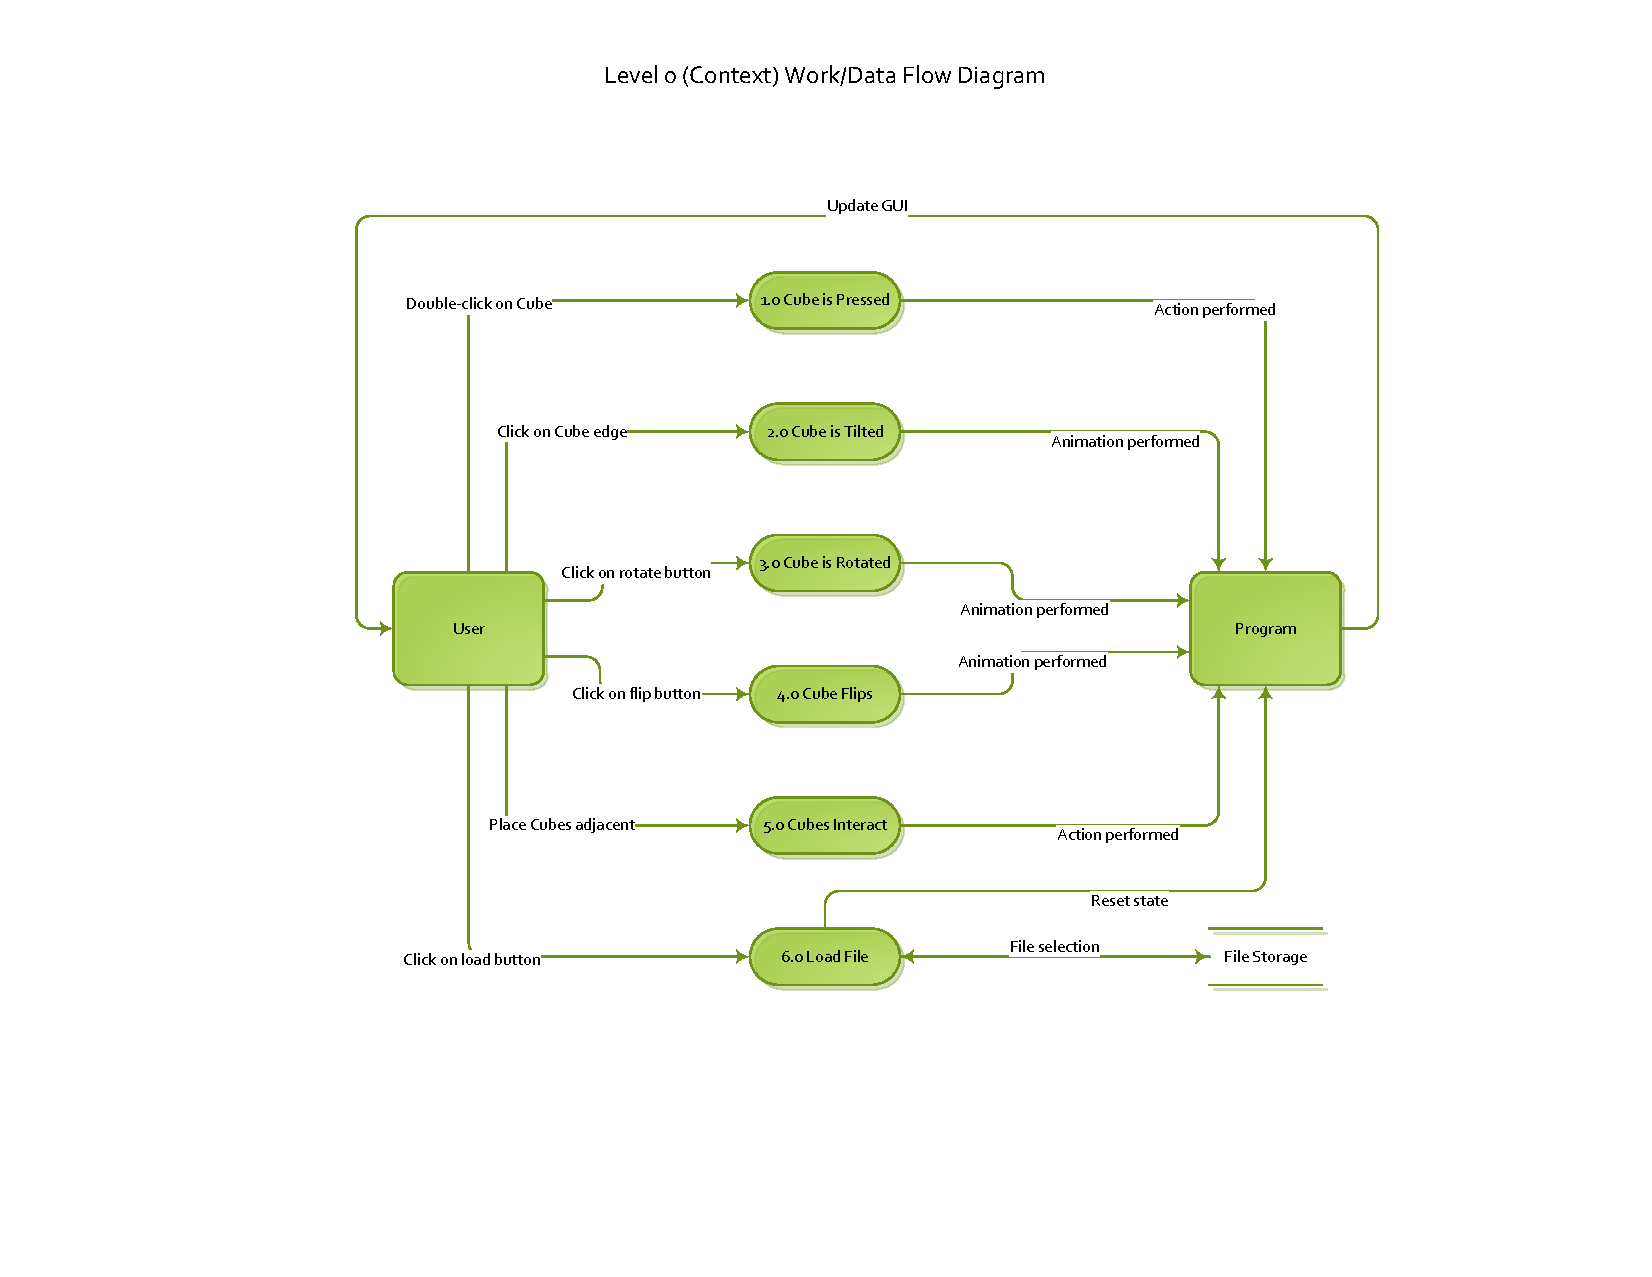
\includepdf[pages={1-7},landscape]{pdfs/dfds.pdf}

\section{Usability Requirements}
The client would like the emulator\index{emulator} to be accessible to new developers, but also efficient for experienced developers to use. The emulator\index{emulator} may have a familiarization time in order for users to be able to use it productively. It will include a help menu containing instructions for the various features. In addition, the client would like keyboard shortcuts and accelerators available for users who prefer keyboard-based controls. As the user must be able to understand how to interact with the Cubes relatively quickly, the Cubes' control motions must be intuitive. The user must also be able to switch between motions quickly.

\section{Performance Requirements}
The performance requirements for the system are fairly basic. When the user interacts with the system there must be no visible graphics delay. Additionally, games simulated on the Cubes must function with performance similar to that of the physical Cubes. Beyond these two key requirements, actions must be performed in a timely manner for all scenarios that may arise during use of the emulator\index{emulator}.

\section{Reliability Requirements}
As a system that emulates another system and runs user-created code, it is important that the Siftables Emulator does not contribute defects of its own to the application testing process. As such, Singularity Software will aim for a defect rate of 5 bugs/KLOC. As a predictor of this result, we will evaluate the cyclomatic complexity of our code at each development milestone, aiming for a score of 15 or less.\footnote{Expected cyclomatic complexity scores are based on the blog post at: http://gdub.wordpress.com/2006/07/09/cyclomatic-complexity-for-python-code/.} When evaluating the reliability of the emulator\index{emulator} prior to release, bugs will be analyzed for priority and severity. For example, misspelled words or other aesthetic issues will not be treated with the same severity as crash-inducing bugs.

\section{Supportability Requirements}
Because all support for Siftables Emulator will be done by the client after the project has ended, it is imperative that the emulator have well-documented code that is easy for developers unfamiliar with the project to follow. It will also need to follow a recognized coding standard for the language chosen. As a result, it must be in an object-oriented language like Python or C\# that is fairly well-known and frequently used.

\section{Hardware and Software Interfaces}
The Siftables Emulator will work as a standalone software package and will not interface with any other software or hardware. Singularity Software considered the integration of the emulator in an \gls{IDE} but decided that the emulator was best served as an independent tool to allow easy development across the supported platforms. Similarly, the purpose of the emulator is to serve as a method for developing applications for the Cubes without connecting to the physical Cubes, so it will not interface with any hardware either.

\section{Documentation, Installation, Legal and Licensing Requirements}
The clients have stated that the emulator project is to be licensed under the BSD 2-clause license\footnote{http://www.opensource.org/licenses/bsd-license.php}; therefore, many of the standard legal and licensing issues are eliminated. Mr. Ekl has requested that Singularity Software keep documentation of development actions according to project milestone standards as well as using error tracking and version tracking systems during the design process. He has also requested that the API developed for the project is documented in a well-accepted form like that produced by Javadoc.\\\\
The emulator\index{emulator} will be installable via an executable (on \gls{Windows}\index{Windows}) or disk image (on \gls{Mac}\index{Mac}) that will place the program's files in a user-specified directory and create shortcuts as appropriate.

\section{Design Constraints}
The emulator\index{emulator} must be able to be function on computers using the \gls{Windows}\index{Windows}, \gls{Mac}\index{Mac} OS, and \gls{Linux}\index{Linux} operating systems that satisfy the minimum system requirements of the previous OS version. In other words, the emulator should run smoothly on a computer that meets the requirements for \gls{Windows}\index{Windows} Vista, \gls{Mac}\index{Mac} OS X 10.6 (Snow Leopard), or Ubuntu 11.04\footnote{The Ubuntu machine should support graphics acceleration (i.e. it should be capable of running the GNOME 3 or Unity window managers).}.

\section{User Interface Mockups}
Preliminary mockups of the Siftables Emulator user interfaces are presented below. The mockups are rough sketches not intended to convey the product's final look. Rather, they present a simplified view of what Singularity thinks the emulator will look like when created in code.\\\\
In order, the mockups display the main screen of the application, the ``Load a program" dialog, and the various warning and alert dialogs that the program can display.\\\\
The Manipulate Cube use case (UC6) is not easily presented in mockup format. Essentially, it applies to any of the 6 Cubes in the first mockup; any of the actions described in the use case can be applied to each virtual Cube.

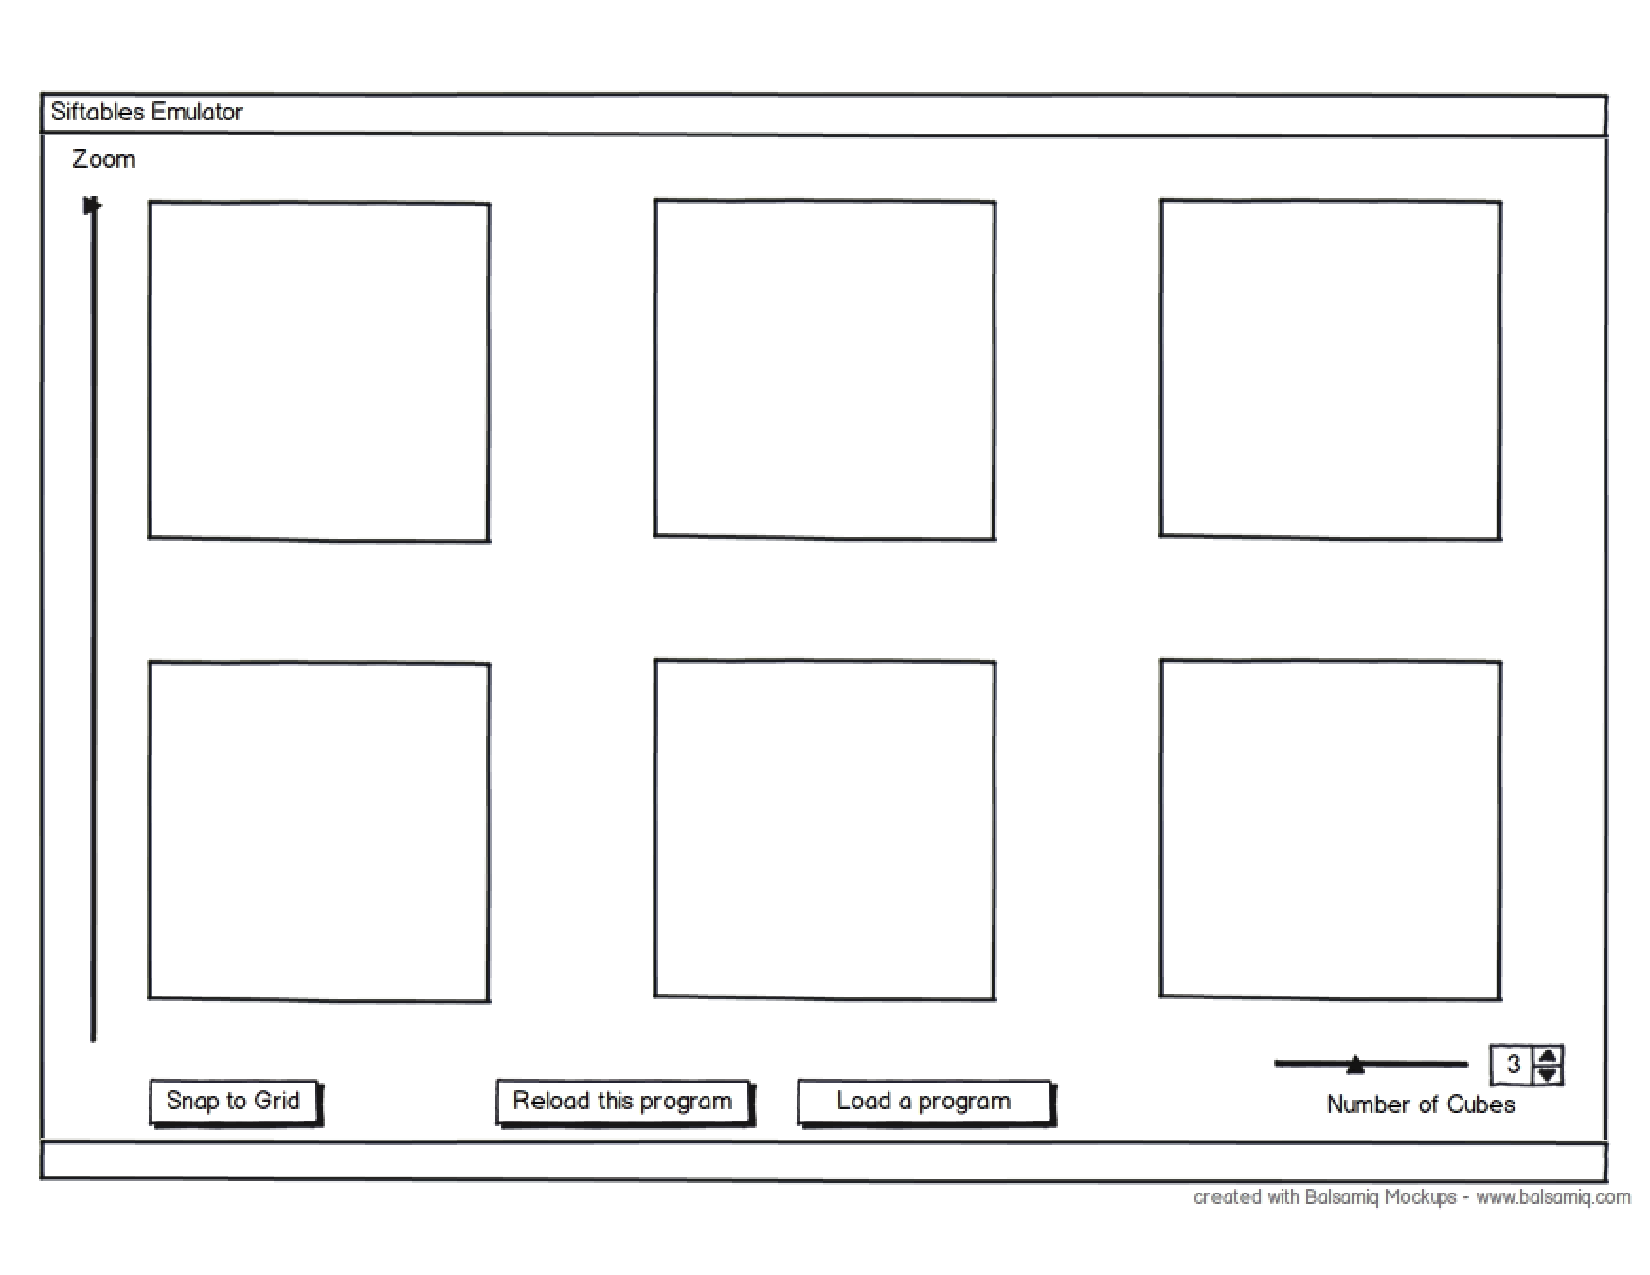
\includepdf[pages={1-3},landscape]{pdfs/mocks.pdf}

\section{Coding Standards}
The developers of Singularity Software will adhere to a standardized coding ``style guide'' based on the language chosen for development. In the case of Python, we will reference the official Style Guide for Python Code [6]. Highlights of that document include 4-space indentation, a lack of extraneous space,  and camel case for class names. In the case of C\#, where no Microsoft-standard coding standards exist, we will use the standards laid out at [7], that emphasize the exclusive use of camel and Pascal case and ANSI-style bracing (where each brace gets its own line).

\section{Change Control}
Change requests may be submitted as issues on the project's GitHub repository\footnote{https://github.com/alexmullans/Siftables-Emulator/issues/new}. At a minimum, requests for change should mention the screen(s) to be changed, the new workflow that is desired (preferably in context with how it differs from the current workflow), the rationale for the change, and the priority the submitter assigns to the change. \\\\
Changes submitted in the manner described will be considered by Singularity during our weekly project meeting. A majority vote (three of four team members) is required to accept a new feature into the system; however, a team member who feels very strongly may exercise a veto on the team's decision. Each team member will receive one veto for every four submitted changes. \\\\
Changes to product documents (i.e. milestones) will be managed using the Git version control framework within which the documents are currently stored. In the case of major changes, the team will consider the use of ``delta'' documents if such documents will be easier to read than heavily modified original documents.

\clearpage
\section{Test Cases}

\subsection{Load program}

\begin{table}[h!]
  \begin{tabular}{l | l | l | l}
    \textbf{Scenario \#} &
    \textbf{Originating Flow} &
    \textbf{Alternate Flow} &
    \textbf{Next Alternate} \\ \hline

    1 &
    Basic flow &
    &
    \\ \hline

    2 &
    Basic flow &
    Alternate flow 1 &
    \\ \hline

    3 &
    Basic flow &
    Alternate flow 2 &
    \\ \hline

    4 &
    Basic flow &
    Alternate flow 3 &
    \\ \hline

    5 &
    Basic flow &
    Alternate flow 4 &
    \\ \hline

    6 &
    Basic flow &
    Alternate flow 4 &
    Basic flow \\ \hline

  \end{tabular}
\end{table}

\begin{table}[h!]
  \begin{tabular}{p{.5in} | p{.75in} | p{2.15in} | p{2.15in}}
    \textbf{Test Case ID} &
    \textbf{Scenario} &
    \textbf{Description} &
    \textbf{Expected Result} \\ \hline

    1 &
    1 &
    A program is successfully loaded in the emulator. &
    The Cubes run the selected program in the Workspace. \\ \hline

    2 &
    2 &
    User selects incompatible file type. &
    ``The selected file is not a .siftem emulator file and cannot be loaded.'' error is displayed. \\ \hline

    3 &
    3 &
    User selects corrupt or unloadable file. &
    ``The selected file is corrupt and cannot be loaded.'' error is displayed. \\ \hline

    4 &
    4 &
    User cancels loading program. &
    The emulator returns to its state before the basic flow was entered. \\ \hline

    5 &
    5 &
    User loads a program when a program is already running and chooses ``Cancel'' on the warning prompt. &
    Emulator returns to its state before the basic flow was entered after ``Cancel'' is chosen. \\ \hline

    6 &
    6 &
    User loads a program when a program is already running and chooses ``Continue" on the warning prompt. &
    Cubes run the selected program in the Workspace after ``Continue'' is chosen. \\ \hline
  \end{tabular}
\end{table}
\clearpage

\subsection{Reload program}

\begin{table}[h!]
  \begin{tabular}{l | l | l}
    \textbf{Scenario \#} &
    \textbf{Originating Flow} &
    \textbf{Alternate Flow} \\ \hline

    1 &
    Basic flow &
    \\ \hline

    2 &
    Basic flow &
    Alternate flow 1 \\ \hline

  \end{tabular}
\end{table}

\begin{table}[h!]
  \begin{tabular}{p{.5in} | p{.75in} | p{2.15in} | p{2.15in}}
    \textbf{Test Case ID} &
    \textbf{Scenario} &
    \textbf{Description} &
    \textbf{Expected Result} \\ \hline

    1 &
    1 &
    The program is successfully reloaded in the emulator. &
    The Cubes run the selected program in the Workspace after the user presses ``Continue'' on the warning message. \\ \hline

    2 &
    2 &
    The user selects ``Cancel'' on the warning dialog (which specifies that the emulator will be reset). &
    The Cubes run the program as originally specified; no change should be made to emulator's state. \\ \hline

  \end{tabular}
\end{table}

\subsection{Zoom screen}

\begin{table}[h!]
  \begin{tabular}{l | l}
    \textbf{Scenario \#} &
    \textbf{Originating Flow} \\ \hline

    1 &
    Basic flow \\ \hline

  \end{tabular}
\end{table}

\begin{table}[h!]
  \begin{tabular}{p{.5in} | p{.75in} | p{2.15in} | p{2.15in}}
    \textbf{Test Case ID} &
    \textbf{Scenario} &
    \textbf{Description} &
    \textbf{Expected Result} \\ \hline

    1 &
    1 &
    User zooms in fully. &
    The Workspace view is centered on the first cube with the edges of the adjacent Cubes visible. \\ \hline

    2 &
    1 &
    User zooms out fully. &
    The entire Workspace is visible. \\ \hline

    3 &
    1 &
    A zoom level in the middle is selected. &
    The slider moves to the closest predefined increment and the correct zoom level is shown. \\ \hline

  \end{tabular}
\end{table}

\clearpage

\subsection{Add/remove Cubes}

\begin{table}[h!]
  \begin{tabular}{l | l | l}
    \textbf{Scenario \#} &
    \textbf{Originating Flow} \\ \hline

    1 &
    Basic flow &
    \\ \hline

  \end{tabular}
\end{table}

\begin{table}[h!]
  \begin{tabular}{p{.5in} | p{.75in} | p{2.15in} | p{2.15in}}
    \textbf{Test Case ID} &
    \textbf{Scenario} &
    \textbf{Description} &
    \textbf{Expected Result} \\ \hline

    1 &
    1 &
    The slider is moved to one of the predefined increments or the spinbox is changed to an integer in the range [1, 6]. &
    The specified number of Cubes is shown in the Workspace. \\ \hline

  \end{tabular}
\end{table}

\subsection{Snap Cubes to grid}

\begin{table}[h!]
  \begin{tabular}{l | l}
    \textbf{Scenario \#} &
    \textbf{Originating Flow} \\ \hline

    1 &
    Basic flow \\ \hline

  \end{tabular}
\end{table}

\begin{table}[h!]
  \begin{tabular}{p{.5in} | p{.75in} | p{2.15in} | p{2.15in}}
    \textbf{Test Case ID} &
    \textbf{Scenario} &
    \textbf{Description} &
    \textbf{Expected Result} \\ \hline

    1 &
    1 &
    User presses the ``Snap to Grid'' button. &
    The emulator aligns the Cubes in a grid based on their current positions.  \\ \hline

  \end{tabular}
\end{table}

\clearpage

\subsection{Manipulate Cube}

\begin{table}[h!]
  \begin{tabular}{l | l}
    \textbf{Scenario \#} &
    \textbf{Originating Flow} \\ \hline

    1 &
    Basic flow \\ \hline

    2 &
    Alternate flow 1 \\ \hline

    3 &
    Alternate flow 2 \\ \hline

    4 &
    Alternate flow 3 \\ \hline

  \end{tabular}
\end{table}

\begin{table}[h!]
  \begin{tabular}{p{.5in} | p{.75in} | p{2.15in} | p{2.15in}}
    \textbf{Test Case ID} &
    \textbf{Scenario} &
    \textbf{Description} &
    \textbf{Expected Result} \\ \hline

    1 &
    1 &
    The user double clicks on a Cube. &
    The Cube responds as if a screen click occured. \\ \hline

    2 &
    2 &
    The user clicks on one of the buttons on the Cube. &
    The Cube executes and responds to the associated action (flip, rotate, or tilt). \\ \hline

    3 &
    3 &
    The user drags a Cube next to another Cube. &
    The Cube neighbors with the adjacent Cube, and the two recognize each other as neighbors. \\ \hline

    4 &
    4 &
    The user drags a Cube back and forth in a shaking manner. &
    The Cube responds as if shaken. \\ \hline

  \end{tabular}
\end{table}

\section{Usability Report}

\subsection{Process}
In order to conduct the usability test, a basic prototype of the Siftables Emulator was developed using Adobe Flash CS5. The prototype, which modeled the basic functionality intended for the final emulator, was then compared to the current Sifteo Inc. emulator, the Siftulator. The tests were conducted using CSSE students and faculty as subjects, because the primary target demographic of the software is developers. \\\\
Participants in the study were first presented with an informed consent form and a pre-test questionnaire that collected relevant personal information. Upon completion of these two documents, the user was then taken into the testing area and given a brief set of verbal instructions by one of the team members. After the team member finished presenting the instructions and left the room, the participant was asked to begin the study by watching a short video demonstrating the capabilities of the Sifteo Cubes. We felt that this was the most efficient way to acquaint users with the product and we believed that it was necessary for them to be able to accurately judge the performance of an emulator. \\\\
Upon completion of the video, participants were asked to complete a series of simple tasks in the current Siftulator platform. Because of the nature of this product and its lack of a help file, a list of action commands from Sifteo's website was located on the table next to the user. If they could not intuitively determine the correct way to complete a task, participants were told that this sheet could be used to help them. Users were then asked to switch to Siftables Emulator prototype and reminded that this product was in no way based on the software which they had just used. They were then asked to complete a similar set of tasks using the prototype. In the event that the user became stuck and was unable to complete their task at any time on either emulator, help was offered. This help was kept to a minimum, often consisting solely of asking the user a question to help them cogitate in a different fashion. \\\\
At the conclusion of the technical portion of the study, participants were thanked for their time and assistance and asked to complete a post-test questionnaire. This questionnaire was designed to allow each user to express his or her opinion about the various aspects of both projects and suggest possible improvements to the interface of the Siftables Emulator prototype.

\subsection{Analysis}
The results from the usability study can be found primarily in the usability report generated by the Ovo software. \\\\
Additionally, a pre-test questionnaire and a post-test questionnaire were distributed to each participant to collect data regarding their overall experience as well as their prior knowledge of the product and similar systems. The informed consent form, pre-test questionnaire, and post-test questionnaire are all included as appendices at the end of this document. The results of the questionnaires are shown in the table following this section. For questions utilizing a Likert scale for answers, the answers were associated with numeric answers, with the most positive answer corresponding to the most positive value.

\subsubsection{Pre-Test Results}
\begin{enumerate}
        \item{All of the participants reported that they had never heard of Sifteo nor their product. This lack of previous experience working with the product provided a clean slate on which to base our findings.}
        \item{All of the participants but one reported having never programmed for an embedded system before. This question does not directly reflect in any of the results, but it indicates that the emulator is still accessible to first-time programmers for embedded systems.}
        \item{\textbf{2.5/4.0}: On average the participants felt somewhere between comfortable and uncomfortable using new software without documentation.  As  that is the exact median of the possible values, these results are expected.}
        \item{\textbf{3.8/4.0}: With documentation, all participants felt at least somewhat comfortable, and all but one reported feeling very comfortable using new software. Because the participants chosen were all from or had experience in the field of computer science/engineering or software engineering, this is expected.}
        \item{\textbf{3.8/4.0}: Similar results were found with the participants' comfort level with using an API.}
        \item{Half of the participants had used an emulator before, and half had not, indicating that our results would accurately depict the user experience on both ends of the spectrum.}
\end{enumerate}

\subsubsection{Study Results}
Results from the usability study with the six participants are available in the usability report. Overall, the times associated with the tasks for Singularity's emulaor were significantly lower than those associated with the tasks for Sifteo's emulator.  \\\\
One notable difference was in the ``Load program'' task.  Using Sifteo's emulator, a user has to open a separate program loader, and navigating to the ``Play'' functionality is not intuitive.  Additionally, there is not much immediate feedback regarding the success of loading a program.  On the other hand, in Singularity's emulator, loading a program was literally as easy as the click of a button, making the task much more straightforward.

\subsubsection{Post-Test Results}
\begin{enumerate}
        \item{\textbf{3.8/4.0}: All but one participant strongly agreed that the main screen of the emulator was accessible. The other participant agreed that the main screen was accessible but did not strongly agree, indicating that the layout works well for efficient use.}
        \item{\textbf{3.7/4.0}: All but two participants strongly agreed, and the other two agreed, that the commands were in easy-to-find locations, reinforcing that the layout of the main screen was well-designed.}
        \item{\textbf{3.1/4.0}: Moving a Cube was not as straightforward; on average, users agreed that it was easy, but one participant strongly disagreed.  Because the moving functionality was not fully implemented in the prototype but participants found it easy to use in Sifteo's emulator, we can ensure that the functionality will be easy to use because we plan on implementing movement in the same way.}
        \item{\textbf{3.4/4.0}: Organizing Cubes on the screen on average was determined to be halfway between agreeing and strongly agreeing. Because only one Cube was present in the emulator, some found it less intuitive because they did not receive visual feedback, which is understandable and does not heavily indicate any lack of usability in the product.}
        \item{\textbf{3.3/4.0}: Manipulating a Cube on average was indicated to be fairly intuitive, but not all functionality was straightforward or immediately obvious.  As the study indicated, shaking and tilting took considerably longer than the other manipulations; some users found the icons associated with these movements unintuitive.}
        \item{\textbf{3.2/4.0}: On average, the participants agreed that Singularity's emulator was easier to use than Sifteo's.  The participants who found Sifteo's emulator easier to use made extensive use of the help sheet provided, so they were able to complete the actions more quickly.}
\end{enumerate}

\begin{landscape}
\begin{center}
  \begin{tabular}{| l | l | l | l | l | l | l | l | l | l | l | l | l | l | l |}
    \hline

    \textbf{Gender} &
    \textbf{Major} &
    \textbf{Class} &
    \textbf{Pre1} &
    \textbf{Pre2} &
    \textbf{Pre3} &
    \textbf{Pre4} &
    \textbf{Pre5} &
    \textbf{Pre6} &
    \textbf{Post1} &
    \textbf{Post2} &
    \textbf{Post3} &
    \textbf{Post4} &
    \textbf{Post5} &
    \textbf{Post6} \\ \hline

    F &
    CS &
    S &
    A &
    No &
    1 &
    4 &
    4 &
    No &
    4 &
    4 &
    1 &
    2 &
    3 &
    3 \\ \hline

    F &
    CE &
    F &
    A &
    No &
    1 &
    3 &
    4 &
    Yes &
    3 &
    4 &
    3 &
    4 &
    3 &
    4 \\ \hline

    M &
    SE/CS/MA &
    S &
    A &
    No &
    3 &
    4 &
    3 &
    Yes &
    4 &
    4 &
    4 &
    4 &
    3 &
    2 \\ \hline

    M &
    SE &
    J &
    A &
    No &
    4 &
    4 &
    4 &
    Yes &
    4 &
    3 &
    4 &
    4 &
    4 &
    2 \\ \hline

    M &
    CSSE &
    Fac &
    A &
    No &
    3 &
    4 &
    4 &
    No &
    4 &
    3 &
    2.5 &
    2.5 &
    3 &
    4 \\ \hline

    M &
    CPE &
    J &
    A &
    Yes &
    3 &
    4 &
    4 &
    No &
    4 &
    4 &
    4 &
    4 &
    4 &
    4 \\ \hline

    & & & & & & & & & & & & & & \\ \hline

    \textbf{Average} &
    & & & &
    2.5 &
    3.8 &
    3.8 &
    &
    3.8 &
    3.7 &
    3.1 &
    3.4 &
    3.3 &
    3.2 \\ \hline

    
  \end{tabular}
\end{center}
\end{landscape}

\subsection{Findings}
Based on the post-test results, our emulator was regarded as having an accessible layout and fairly intuitive controls.  All the users at least agreed that the commands were in easy-to-find locations and that the main screen looked accessible. \\\\
One aspect that the users saw could be improved is manipulating the Cube.  While rotating and flipping were not an issue for most users, they found tilting and shaking to be more difficult to comprehend.  For this reason, we made the edges of the Cube bolder to help inform the user where to grab the Cube for tilting and also changed the shake icon to be more recognizable.  However, since most of the users’ first instinct to shake the Cube was to drag it with the mouse, the shake icon is temporary and we plan to implement mouse control for the shake command in the future. \\\\
Users, on average, completed the designated tasks quicker and with less help in comparison to Sifteo’s emulator.  Overall, the emulator was viewed as an improvement over Sifteo’s emulator by outperforming it in various tasks such as adding/removing Cubes, loading programs, and controlling the Cubes.

\section{Interaction Architecture}
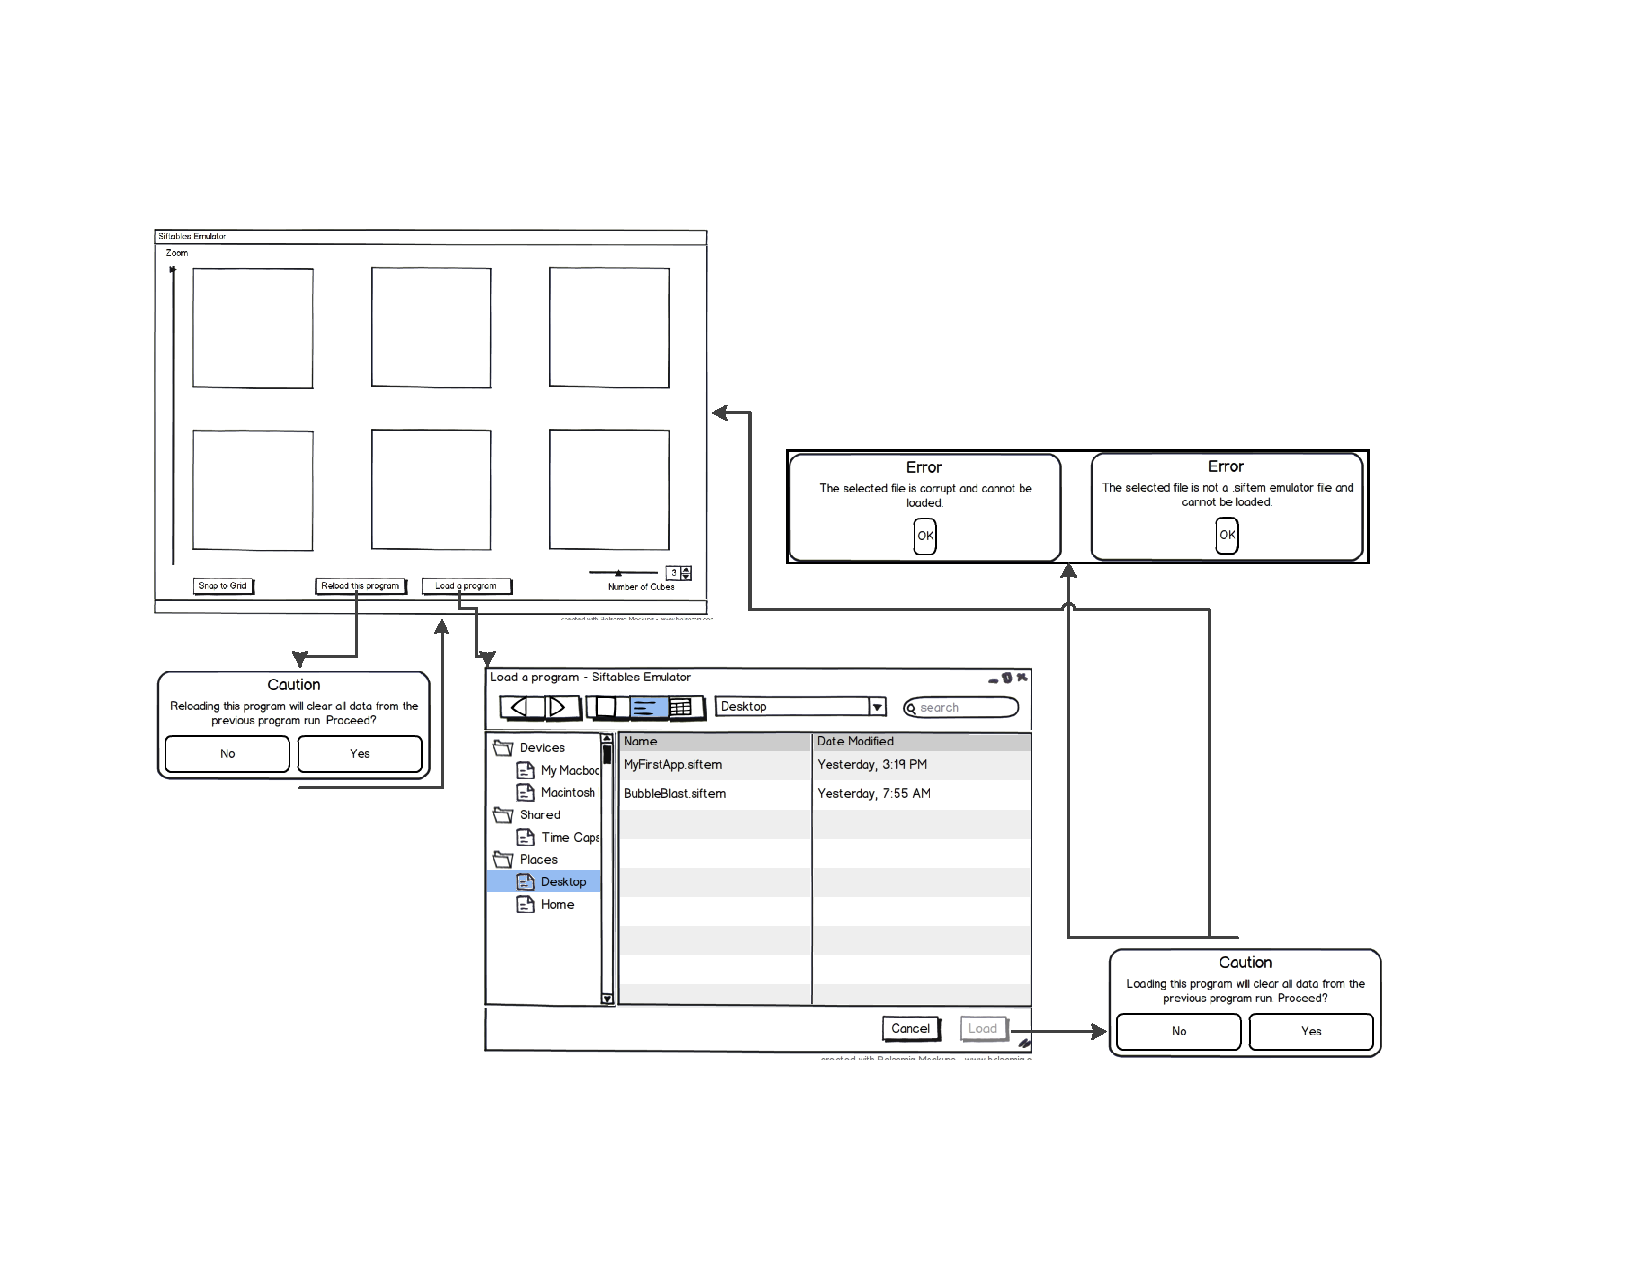
\includepdf[landscape]{interaction.pdf}

\section{Initial Interface Design}
\begin{center}
  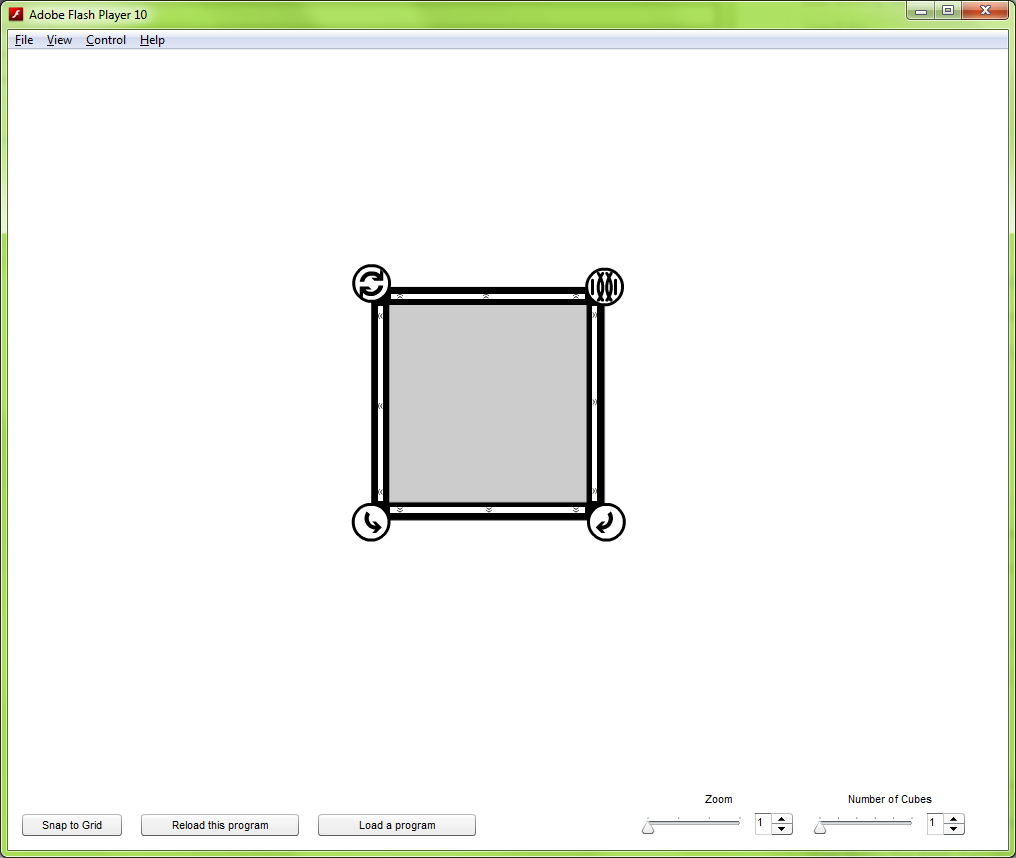
\includegraphics[scale=.4]{../prototype/prototype1.png}
\end{center}

Singularity's initial interface design was well-received. Usability testers were able to easily access all presented functions except tilt and shake.

\section{Revised Interface Design}
\begin{center}
  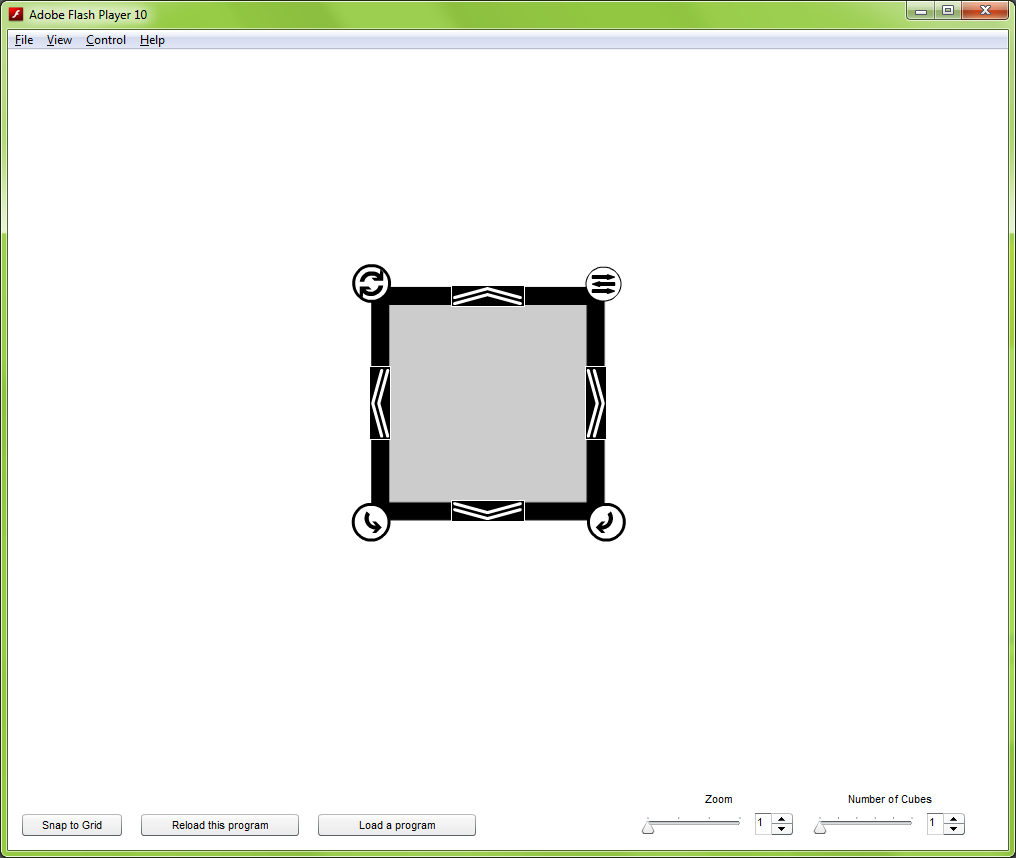
\includegraphics[scale=.4]{../prototype/prototype2.png}
\end{center}

Based on the results of the usability test, Singularity redesigned parts of the interface to make the tilt and shake actions more obvious. Specifically, we replaced the tilt buttons on each side of the cube with larger, clearer instances. Additionally, we redesigned the shake button to increase its clarity and better relate the icon to the button's purpose.

\clearpage
\addcontentsline{toc}{section}{Glossary}
\printglossaries
\clearpage

\addcontentsline{toc}{section}{References}
\section*{References}

        \begin{enumerate}
                \item{Sifteo Inc. Online: http://www.sifteo.com}
                \item{Tim Ekl.  Client Meeting. 25 October 2011 2:30 p.m.}
                \item{Milestone 1.  Singularity Software.  Online: https://github.com/alexmullans/Siftables-Emulator/blob/master/docs/pdfs/m1.pdf}
                \item{Milestone 2.  Singularity Software.  Online: https://github.com/alexmullans/Siftables-Emulator/blob/master/docs/pdfs/m2.pdf}
                \item{Milestone 3.  Singularity Software.  Online: https://github.com/alexmullans/Siftables-Emulator/blob/master/docs/pdfs/m3.pdf}
                \item{Milestone 4.  Singularity Software.  Online: https://github.com/alexmullans/Siftables-Emulator/blob/master/docs/pdfs/m4.pdf}

        \end{enumerate}
        
\clearpage

\addcontentsline{toc}{section}{Index}
\printindex
        
\end{document}
